\chapter{LEVEL 19+ @Problem 475+}
\section{Problem 476}
\begin{prob}
\end{prob}

\section{Problem 479 - Roots on the Rise}
\begin{prob}
	\begin{figure}[htb!]
		\begin{center}
			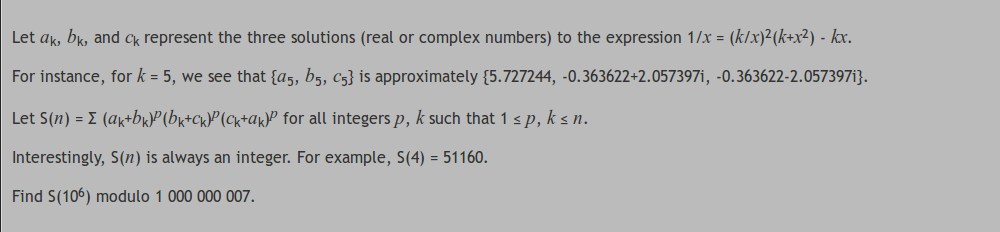
\includegraphics[scale = 0.4]{pic/479.png}
		\end{center}
	\end{figure}
\end{prob}
\begin{sol}
By Vieta's formulas, $a_k + b_k + c_k = k$, $a_kb_k + b_kc_k + c_ka_k = 1/k$, $a_kb_kc_k = k^2$.
\begin{eqnarray}
(a_k + b_k)(b_k + c_k)(c_k + a_k) = (a_k + b_k + c_k)(a_kb_k + b_kc_k + c_ka_k) -a_kb_kc_k = 1 - k^2.
\end{eqnarray}
Then we just have to evaluate
\begin{eqnarray}
\sum_{k = 1}^n ((1 - k^2)^{n + 1} - (1 - k^2))/(- k^2) \mod p
\end{eqnarray}
where 
\begin{eqnarray}
(-k^2)^{-1} \equiv (-k^2)^{p-2} \mod{p}
\end{eqnarray}
Using \texttt{ModPow} with \texttt{BigInt} will be efficient, in \texttt{Python}, simply use \texttt{pow} with the third argument.
\code{code/479.py}
\end{sol}
\section{Problem 500}
\begin{prob}
\end{prob}